% Execution model on the OSPool: one HTCondor job = one (ensemble, stream segment | config, task).
\documentclass[tikz,border=8pt]{standalone}
\usetikzlibrary{arrows.meta,calc}
\definecolor{ink}{HTML}{222222}
\definecolor{acc}{HTML}{B2182B}
\definecolor{blu}{HTML}{2166AC}
\definecolor{gold}{HTML}{C8961E}
\tikzset{
  box/.style={draw=ink!60, line width=0.5pt, rounded corners=2pt, align=center, font=\footnotesize,
              inner sep=4pt, minimum height=1.0cm, minimum width=3.3cm, fill=white},
  gpu/.style={box, draw=acc, fill=acc!5},
  cpu/.style={box, draw=blu, fill=blu!5},
  store/.style={box, draw=gold!70!black, fill=gold!8},
  arr/.style={-{Stealth[length=4pt]}, line width=0.5pt, draw=ink!65},
  lbl/.style={font=\scriptsize, text=ink!60},
}
\begin{document}
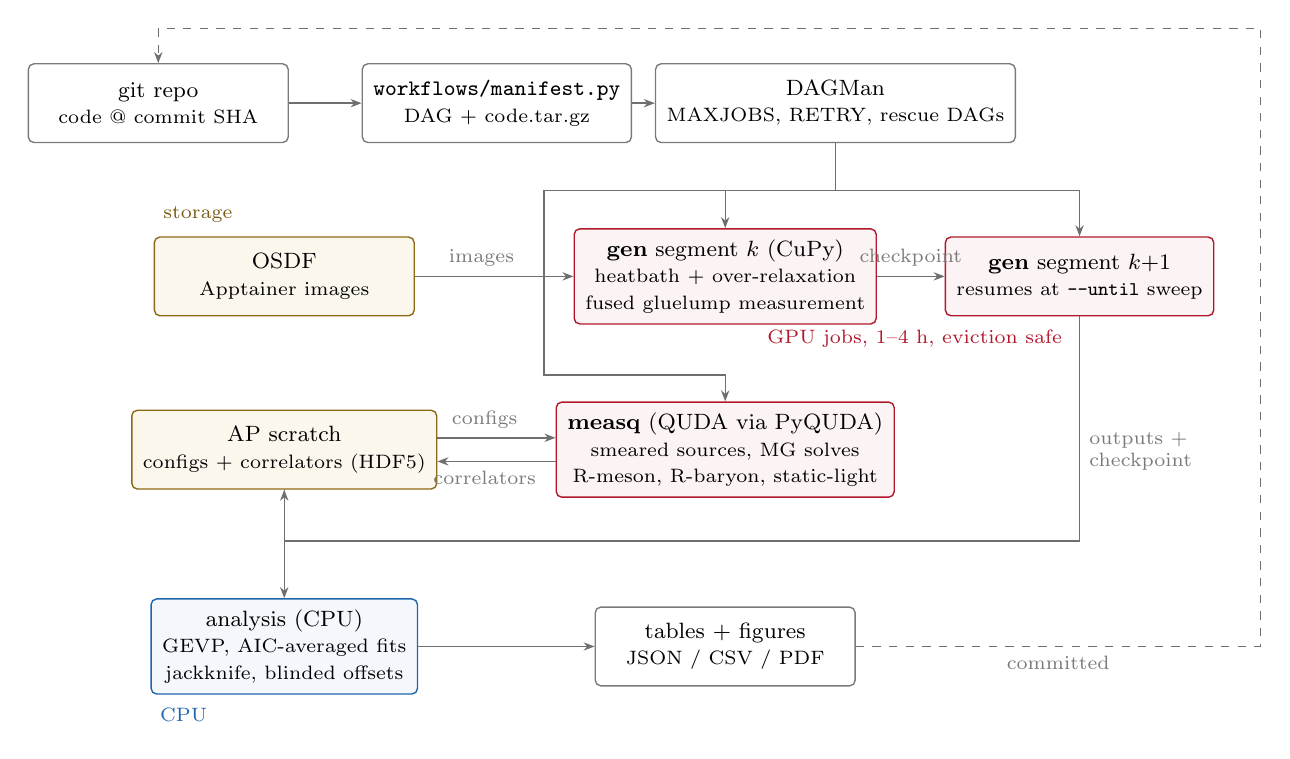
\begin{tikzpicture}
  % row 1: control
  \node[box] (git) at (0,0) {git repo\\\scriptsize code @ commit SHA};
  \node[box] (man) at (4.3,0) {\texttt{workflows/manifest.py}\\\scriptsize DAG + code.tar.gz};
  \node[box] (dag) at (8.6,0) {DAGMan\\\scriptsize MAXJOBS, RETRY, rescue DAGs};
  \draw[arr] (git) -- (man);
  \draw[arr] (man) -- (dag);
  % row 2: GPU jobs
  \node[gpu] (gen) at (7.2,-2.2) {\textbf{gen} segment $k$ (CuPy)\\\scriptsize heatbath + over-relaxation\\\scriptsize fused gluelump measurement};
  \node[gpu] (gen2) at (11.7,-2.2) {\textbf{gen} segment $k{+}1$\\\scriptsize resumes at \texttt{--until} sweep};
  \node[gpu] (meas) at (7.2,-4.4) {\textbf{measq} (QUDA via PyQUDA)\\\scriptsize smeared sources, MG solves\\\scriptsize R-meson, R-baryon, static-light};
  \draw[arr] (dag.south) -- ++(0,-0.6) -| (gen.north);
  \draw[arr] (dag.south) -- ++(0,-0.6) -| (gen2.north);
  \draw[arr] (dag.south) -- ++(0,-0.6) -| (4.9,-3.45) -| (meas.north);
  \draw[arr] (gen) -- node[lbl, above]{checkpoint} (gen2);
  % storage column
  \node[store] (osdf) at (1.6,-2.2) {OSDF\\\scriptsize Apptainer images};
  \node[store] (scr) at (1.6,-4.4) {AP scratch\\\scriptsize configs + correlators (HDF5)};
  \draw[arr] (osdf) -- node[lbl, above, pos=0.42]{images} (gen);
  \draw[arr] (scr.east) ++(0,0.15) -- node[lbl, above, pos=0.4]{configs} ($(meas.west)+(0,0.15)$);
  \draw[arr] ($(meas.west)+(0,-0.15)$) -- node[lbl, below, pos=0.6]{correlators} ($(scr.east)+(0,-0.15)$);
  \draw[arr] (gen2.south) |- node[lbl, pos=0.3, right, align=left]{outputs +\\checkpoint} ($(meas.south)+(0,-0.55)$) -| (scr.south);
  % row 4: analysis
  \node[cpu] (ana) at (1.6,-6.9) {analysis (CPU)\\\scriptsize GEVP, AIC-averaged fits\\\scriptsize jackknife, blinded offsets};
  \node[box] (fig) at (7.2,-6.9) {tables + figures\\\scriptsize JSON / CSV / PDF};
  \draw[arr] (scr) -- (ana);
  \draw[arr] (ana) -- (fig);
  \draw[arr, dashed] (fig.east) -- (14.0,-6.9) node[lbl, pos=0.5, below]{committed} -- (14.0,0.95) -| (git.north);
  % direct colour key
  \node[lbl, text=acc, anchor=north east] at ($(gen2.south)+(-0.1,-0.05)$) {GPU jobs, 1--4 h, eviction safe};
  \node[lbl, text=gold!60!black, anchor=south west] at ($(osdf.north west)+(0,0.05)$) {storage};
  \node[lbl, text=blu, anchor=north west] at ($(ana.south west)+(0,-0.05)$) {CPU};
\end{tikzpicture}
\end{document}
